\hypertarget{user_8cpp}{}\section{src/user.cpp File Reference}
\label{user_8cpp}\index{src/user.\+cpp@{src/user.\+cpp}}


\hyperlink{classUser}{User} constructor.  


{\ttfamily \#include $<$iostream$>$}\newline
{\ttfamily \#include $<$cstring$>$}\newline
{\ttfamily \#include $<$string$>$}\newline
{\ttfamily \#include \char`\"{}user.\+h\char`\"{}}\newline
{\ttfamily \#include \char`\"{}crypt.\+h\char`\"{}}\newline
{\ttfamily \#include \char`\"{}exception.\+h\char`\"{}}\newline
{\ttfamily \#include $<$stdio.\+h$>$}\newline
Include dependency graph for user.\+cpp\+:
\nopagebreak
\begin{figure}[H]
\begin{center}
\leavevmode
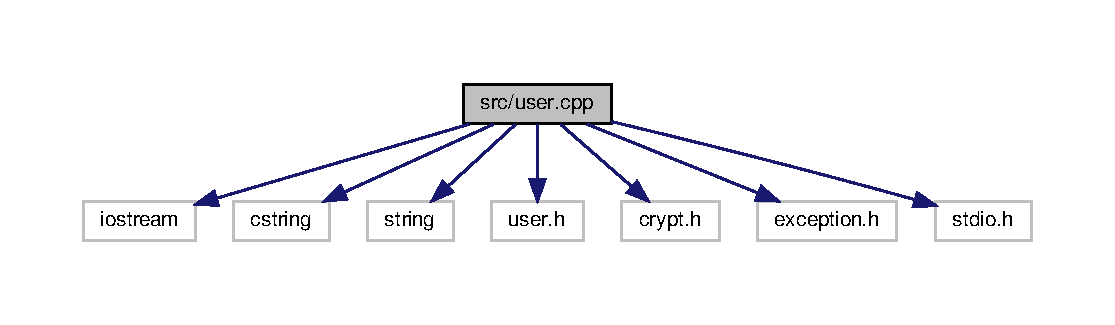
\includegraphics[width=350pt]{user_8cpp__incl}
\end{center}
\end{figure}


\subsection{Detailed Description}
\hyperlink{classUser}{User} constructor. 

Sets the National Insurance number.

Sets the National Insurance number of the user.

Hashes the password.

Signs the user out.

Signs in a user.

Sets the account type of the user.

Sets the country of the user.

Sets the province of the user.

Sets the city of the user.

Sets the email address of the user.

Sets the phone number of the user.

Sets the address of the user.

Sets the first name of the user.

Sets the password.

Sets the username.

Gets the type of account.

Gets user\textquotesingle{}s country.

Gets email address.

Gets phone number.

Gets postcode.

Gets province.

Gets city.

Gets address.

Gets surname.

Gets first name of user.

Gets password.

Gets username.

\hyperlink{classUser}{User()}

\begin{DoxyAuthor}{Author}
Matthew Boote
\end{DoxyAuthor}
Creates new database object \begin{DoxyVerb}@param[in] std::string cname        Company name

@param[out] None

@return None\end{DoxyVerb}


Get\+Username()

\begin{DoxyAuthor}{Author}
Matthew Boote
\end{DoxyAuthor}
Gets username attribute \begin{DoxyVerb}@param[in] None

@param[out] None

@return std::string company name\end{DoxyVerb}


Get\+Password()

\begin{DoxyAuthor}{Author}
Matthew Boote
\end{DoxyAuthor}
Gets password from user object \begin{DoxyVerb}@param[in] None

@param[out] None

@return std::string password\end{DoxyVerb}


Get\+Firstname()

\begin{DoxyAuthor}{Author}
Matthew Boote
\end{DoxyAuthor}
Gets first name from object \begin{DoxyVerb}@param[in] None

@param[out] None

@return std::string firstname\end{DoxyVerb}


Get\+Surname()

\begin{DoxyAuthor}{Author}
Matthew Boote
\end{DoxyAuthor}
Gets surname from user object \begin{DoxyVerb}@param[in] None

@param[out] None

@return std::string surname\end{DoxyVerb}


Get\+Address()

\begin{DoxyAuthor}{Author}
Matthew Boote
\end{DoxyAuthor}
Gets address from user object \begin{DoxyVerb}@param[in] None

@param[out] None

@return std::string address\end{DoxyVerb}


Get\+City()

\begin{DoxyAuthor}{Author}
Matthew Boote
\end{DoxyAuthor}
Gets city from user object \begin{DoxyVerb}@param[in] None

@param[out] None

@return std::string city\end{DoxyVerb}


Get\+Province()

\begin{DoxyAuthor}{Author}
Matthew Boote
\end{DoxyAuthor}
Gets province from user object \begin{DoxyVerb}@param[in] None

@param[out] None

@return std::string province\end{DoxyVerb}


Get\+Postcode()

\begin{DoxyAuthor}{Author}
Matthew Boote
\end{DoxyAuthor}
Gets postcode from user object \begin{DoxyVerb}@param[in] None

@param[out] None

@return std::string postcode\end{DoxyVerb}


Get\+Province()

\begin{DoxyAuthor}{Author}
Matthew Boote
\end{DoxyAuthor}
Gets phone number from user object \begin{DoxyVerb}@param[in] None

@param[out] None

@return std::string phonenumber\end{DoxyVerb}


Get\+Email()

\begin{DoxyAuthor}{Author}
Matthew Boote
\end{DoxyAuthor}
Gets email address from user object \begin{DoxyVerb}@param[in] None

@param[out] None

@return std::string email\end{DoxyVerb}


Get\+Country()

\begin{DoxyAuthor}{Author}
Matthew Boote
\end{DoxyAuthor}
Gets country from user object \begin{DoxyVerb}@param[in] None

@param[out] None

@return std::string country\end{DoxyVerb}


Get\+Province()

\begin{DoxyAuthor}{Author}
Matthew Boote
\end{DoxyAuthor}
Gets the type of user (\hyperlink{classCargoOwner}{Cargo\+Owner}, \hyperlink{classDriver}{Driver} or Transportation\+Company) \begin{DoxyVerb}@param[in] None

@param[out] None

@return std::string usertype\end{DoxyVerb}


Set\+Username()

\begin{DoxyAuthor}{Author}
Matthew Boote
\end{DoxyAuthor}
Sets the username in the object \begin{DoxyVerb}@param[in] std::string username

@param[out] None

@return None\end{DoxyVerb}


Set\+Password()

\begin{DoxyAuthor}{Author}
Matthew Boote
\end{DoxyAuthor}
Sets the password in the object \begin{DoxyVerb}@param[in] std::string password

@param[out] None

@return None\end{DoxyVerb}


Set\+Firstname()

\begin{DoxyAuthor}{Author}
Matthew Boote
\end{DoxyAuthor}
Sets the first name in the object \begin{DoxyVerb}@param[in] std::string user

@param[out] None

@return None\end{DoxyVerb}


Set\+Surname()

\begin{DoxyAuthor}{Author}
Matthew Boote
\end{DoxyAuthor}
Sets the first name in the object/ \begin{DoxyVerb}@param[in] std::string sname

@param[out] None

@return None\end{DoxyVerb}


Set\+Address()

\begin{DoxyAuthor}{Author}
Matthew Boote
\end{DoxyAuthor}
Sets the address in the object \begin{DoxyVerb}@param[in] std::string user

@param[out] None

@return None\end{DoxyVerb}


Set\+Firstname()

\begin{DoxyAuthor}{Author}
Matthew Boote
\end{DoxyAuthor}
Sets the first name in the object/ \begin{DoxyVerb}@param[in] std::string user

@param[out] None

@return None\end{DoxyVerb}


Set\+Firstname()

\begin{DoxyAuthor}{Author}
Matthew Boote
\end{DoxyAuthor}
Sets the phone number in the object/ \begin{DoxyVerb}@param[in] std::string phonenumber

@param[out] None

@return None\end{DoxyVerb}


Set\+Email()

\begin{DoxyAuthor}{Author}
Matthew Boote
\end{DoxyAuthor}
Sets the email address in the object/ \begin{DoxyVerb}@param[in] std::string emailaddress

@param[out] None

@return None\end{DoxyVerb}


Set\+City()

\begin{DoxyAuthor}{Author}
Matthew Boote
\end{DoxyAuthor}
Sets the city in the object \begin{DoxyVerb}@param[in] std::string newcity

@param[out] None

@return None\end{DoxyVerb}


Set\+Province()

\begin{DoxyAuthor}{Author}
Matthew Boote
\end{DoxyAuthor}
Sets the province in the object \begin{DoxyVerb}@param[in] std::string newprovince

@param[out] None

@return None\end{DoxyVerb}


Set\+Country()

\begin{DoxyAuthor}{Author}
Matthew Boote
\end{DoxyAuthor}
Sets the country in the object \begin{DoxyVerb}@param[in] std::string state

@param[out] None

@return None\end{DoxyVerb}


Set\+Account\+Type()

\begin{DoxyAuthor}{Author}
Matthew Boote
\end{DoxyAuthor}
Sets the account type (\hyperlink{classCargoOwner}{Cargo\+Owner}, \hyperlink{classDriver}{Driver}, Transportation\+Company) \begin{DoxyVerb}@param[in] std::string atype

@param[out] None

@return None\end{DoxyVerb}


Sign\+In()

\begin{DoxyAuthor}{Author}
Matthew Boote
\end{DoxyAuthor}
Sign\+In user reads the user account details from the user database, and compares them to the username and password. If the username and password match, it loads the information into the object. \begin{DoxyVerb}@param[in] std::string user

@param[out] None

@return true or false\end{DoxyVerb}


Sign\+Out()

\begin{DoxyAuthor}{Author}
Matthew Boote
\end{DoxyAuthor}
Signs the user out \begin{DoxyVerb}@param[in] None

@param[out] None

@return boolean\end{DoxyVerb}


Hash\+Password

\begin{DoxyAuthor}{Author}
Matthew Boote
\end{DoxyAuthor}
The function hash the password with the U\+N\+IX crypt() function using the username as the salt. It converts the salt and password to char $\ast$, hashes the password and converts it back \begin{DoxyVerb}@param[in] std::string salt,std::string password

@param[out] None

@return None\end{DoxyVerb}


Set\+N\+I\+Number()

\begin{DoxyAuthor}{Author}
Matthew Boote
\end{DoxyAuthor}

\begin{DoxyParams}[1]{Parameters}
\mbox{\tt in}  & {\em std\+::string} & ni\\
\hline
\mbox{\tt out}  & {\em None} & \\
\hline
\end{DoxyParams}
\begin{DoxyReturn}{Returns}
None
\end{DoxyReturn}
Get\+N\+I\+Number()

\begin{DoxyAuthor}{Author}
Matthew Boote
\end{DoxyAuthor}

\begin{DoxyParams}[1]{Parameters}
\mbox{\tt in}  & {\em std\+::string} & user\\
\hline
\mbox{\tt out}  & {\em None} & \\
\hline
\end{DoxyParams}
\begin{DoxyReturn}{Returns}
None 
\end{DoxyReturn}
